\documentclass[12pt]{article}
\usepackage{fullpage,psfrag,amsmath,amsfonts,verbatim,mathtools,scrextend}
\usepackage[small,bf]{caption}

\usepackage[framed,numbered]{mcode}

\usepackage[applemac]{inputenc}
\usepackage[T1]{fontenc}

\usepackage{url}

\usepackage[demo]{graphicx}
\usepackage{subfigure}
\usepackage{xcolor}

\usepackage{enumerate}

\bibliographystyle{alpha}

\title{Optimization and Algorithms \\ Project report}
\author{Group 42 \\ Jos{\'e} Neves 89683, Leonardo Duarte 89691, and Gustavo Bakker 100660}
\date{}

\begin{document}
\maketitle

\section{Part 1}

\section{Part 2}

\subsection{Task 1}

In this Part, the goal is to solve the optimization problem
\begin{equation} \label{eq:problem}
    \begin{array}[t]{ll} 
        \underset{(s,r) \in \mathbf{R}^n \times \mathbf{R}}{\text{minimize}} & \frac{1}{K} \sum_{k=1}^{K} \left(\log \left (1+\exp \left (s^T x_k - r\right) \right) - y_k \left (s^T x_k - r\right)  \right).\\
    \end{array} 
\end{equation}
From \eqref{eq:problem}, the objective function is $f: {\mathbf R}^n \times {\mathbf R} \rightarrow {\mathbf R}$
\begin{equation} \label{eq:objective_function_task_1}
    f(s,r) = \frac{1}{K} \sum_{k=1}^{K} \left(\log \left (1+\exp \left (s^T x_k - r\right) \right) - y_k \left (s^T x_k - r\right)  \right),
\end{equation}
which can be written as
\begin{equation} \label{eq:hk_lk_decomposition}
    f(s,r) = \sum_{k=1}^{K} \frac{1}{K} h_k(s,r) + \sum_{k=1}^{K} \frac{1}{K} l_k(s,r),
\end{equation}
where, for $k=1,...,K$, $h_k:{\mathbf R}^n \times {\mathbf R} \rightarrow {\mathbf R}$
\begin{equation} \label{eq:hk_0}
    h_k(s,r)=\log \left(1+\exp \left(s^T x_k - r\right)\right),
\end{equation}
and $l_k:{\mathbf R}^n \times {\mathbf R} \rightarrow {\mathbf R}$
\begin{equation} \label{eq:lk}
    l_k(s,r)=-y_k \left (s^T x_k - r\right).
\end{equation}
From \eqref{eq:lk}, the functions $l_k$ can be written as
\begin{equation}
    l_k(s,r) = \begin{bmatrix}
        -y_k x_k \\
        y_k
    \end{bmatrix}^T
    \begin{bmatrix}
        s \\
        r
    \end{bmatrix} + 0,
\end{equation}
Therefore, the functions $l_k$ are affine. Since $l_k$ are affine, they are also convex. In addition, from \eqref{eq:hk_0}, the functions $h_k$ can be written as
\begin{equation} \label{eq:hk}
    h_k(s,r) = \left (t_k \circ q_k \right) (s,r),
\end{equation}
where, for $k=1,...,K$, $t_k: {\mathbf R} \rightarrow {\mathbf R}$
\begin{equation} \label{eq:tk}
    t_k(z) = \log(1+\exp(z))
\end{equation}
and $q_k: {\mathbf R}^n \times {\mathbf R} \rightarrow {\mathbf R}$
\begin{equation} \label{eq:qk}
    q_k(z) = s^T x_k - r.
\end{equation}
From \eqref{eq:tk}, it can be observed that the functions $t_k$ are logistic functions and, therefore, convex. The functions $q_k$, in the other hand, can be written from \eqref{eq:qk} as
\begin{equation*}
    q_k (s,r) =
    \begin{bmatrix}
    x_k \\
    -1
    \end{bmatrix}^T
    \begin{bmatrix}
    s \\
    r
    \end{bmatrix} + 0,
\end{equation*}
being, therefore, affine. Since the functions $q_k$ are affine and $t_k$ are convex, it is know from \eqref{eq:hk} that each function $h_k$ can be written as the composition of an affine function with a convex function, which means the functions $h_k$ are all convex. Since all functions $h_k$ and $l_k$ are convex, it is also known from \eqref{eq:objective_function_task_1} that the objective function $f$ is the sum with positive coefficients of convex functions, which means $f$ is convex.

\subsection{Task 2}

In this Task, the gradient descent algorithm will be used to solve \eqref{eq:problem}. To use this algorithm, it is necessary to know the gradient of $f$. From \eqref{eq:hk_lk_decomposition}, one can write
\begin{equation} \label{eq:gradient}
    \nabla f(s,r) = \frac{1}{K} \sum_{k=1}^K (\nabla h_k(s,r) + \nabla l_k(s,r)).
\end{equation}
From \eqref{eq:lk}, the gradient of $l_k$ can be written as
\begin{equation} \label{eq:lk_gradient}
    \nabla l_k (s,r) = 
    \begin{bmatrix}
    -y_k x_k \\
    y_k \\
    \end{bmatrix} = 
    -y_k \begin{bmatrix}
    x_k \\
    -1
    \end{bmatrix}.
\end{equation}
From \eqref{eq:hk}, it can be written that
\begin{equation} \label{eq:hk_composition_gradient}
    \nabla h_k(s,r) = \nabla t_k (q_k(s,r)) \nabla q_k(s,r),
\end{equation}
where, from \eqref{eq:qk},
\begin{equation} \label{eq:qk_gradient}
    \nabla q_k (s,r) =
    \begin{bmatrix}
    x_k \\
    -1
    \end{bmatrix}
\end{equation}
and, from \eqref{eq:tk},
\begin{equation} \label{eq:tk_gradient}
    \nabla t_k(z) = \dfrac{d t_k}{d z} (z) = \frac{\exp(z)}{1+\exp(z)}.
\end{equation}
Combining \eqref{eq:qk}, \eqref{eq:hk_composition_gradient}, \eqref{eq:qk_gradient}, and \eqref{eq:tk_gradient} leads to
\begin{equation} \label{eq:hk_gradient}
    \nabla h_k (s,r) = \left (1 - \frac{1}{\exp \left(
    \begin{bmatrix}
    x_k \\
    -1
    \end{bmatrix}^T
    \begin{bmatrix}
    s \\
    r
    \end{bmatrix}
    \right) + 1} \right)
    \begin{bmatrix}
    x_k \\
    -1
    \end{bmatrix}.
\end{equation}
Finally, combining \eqref{eq:gradient}, \eqref{eq:lk_gradient}, and \eqref{eq:hk_gradient}, one can write
\begin{equation} \label{eq:gradient_final}
    \nabla f (s,r) = \frac{1}{K} \sum_{k=1}^K \left (1 - y_k - \frac{1}{\exp \left(
    \begin{bmatrix}
    x_k \\
    -1
    \end{bmatrix}^T
    \begin{bmatrix}
    s \\
    r
    \end{bmatrix}
    \right) + 1} \right)
    \begin{bmatrix}
    x_k \\
    -1
    \end{bmatrix}.
\end{equation}

In order to apply the gradient method, the following MATLAB script was written. This script returns the results of the method for each of the datasets given. This script implements the Gradient Descent algorithm through the MATLAB function \textit{gradientDescent} also given below.

\lstinputlisting{code/GradientMethod.m}

\lstinputlisting{code/gradientDescent.m}

For Task 2, the results obtained were $s=(1.3495,1.0540)$ and $r=4.8815$. The dataset 1 and the line defined by $\{ x \in \mathbf{R}^2: s^T x = r\}$ are represented in Fig. \ref{fig:GD_dataset1}. In Fig. \ref{fig:GD_norm_dataset1}, the norm of the gradient along iterations is represented.

\begin{figure}[ht!]
    \centering
    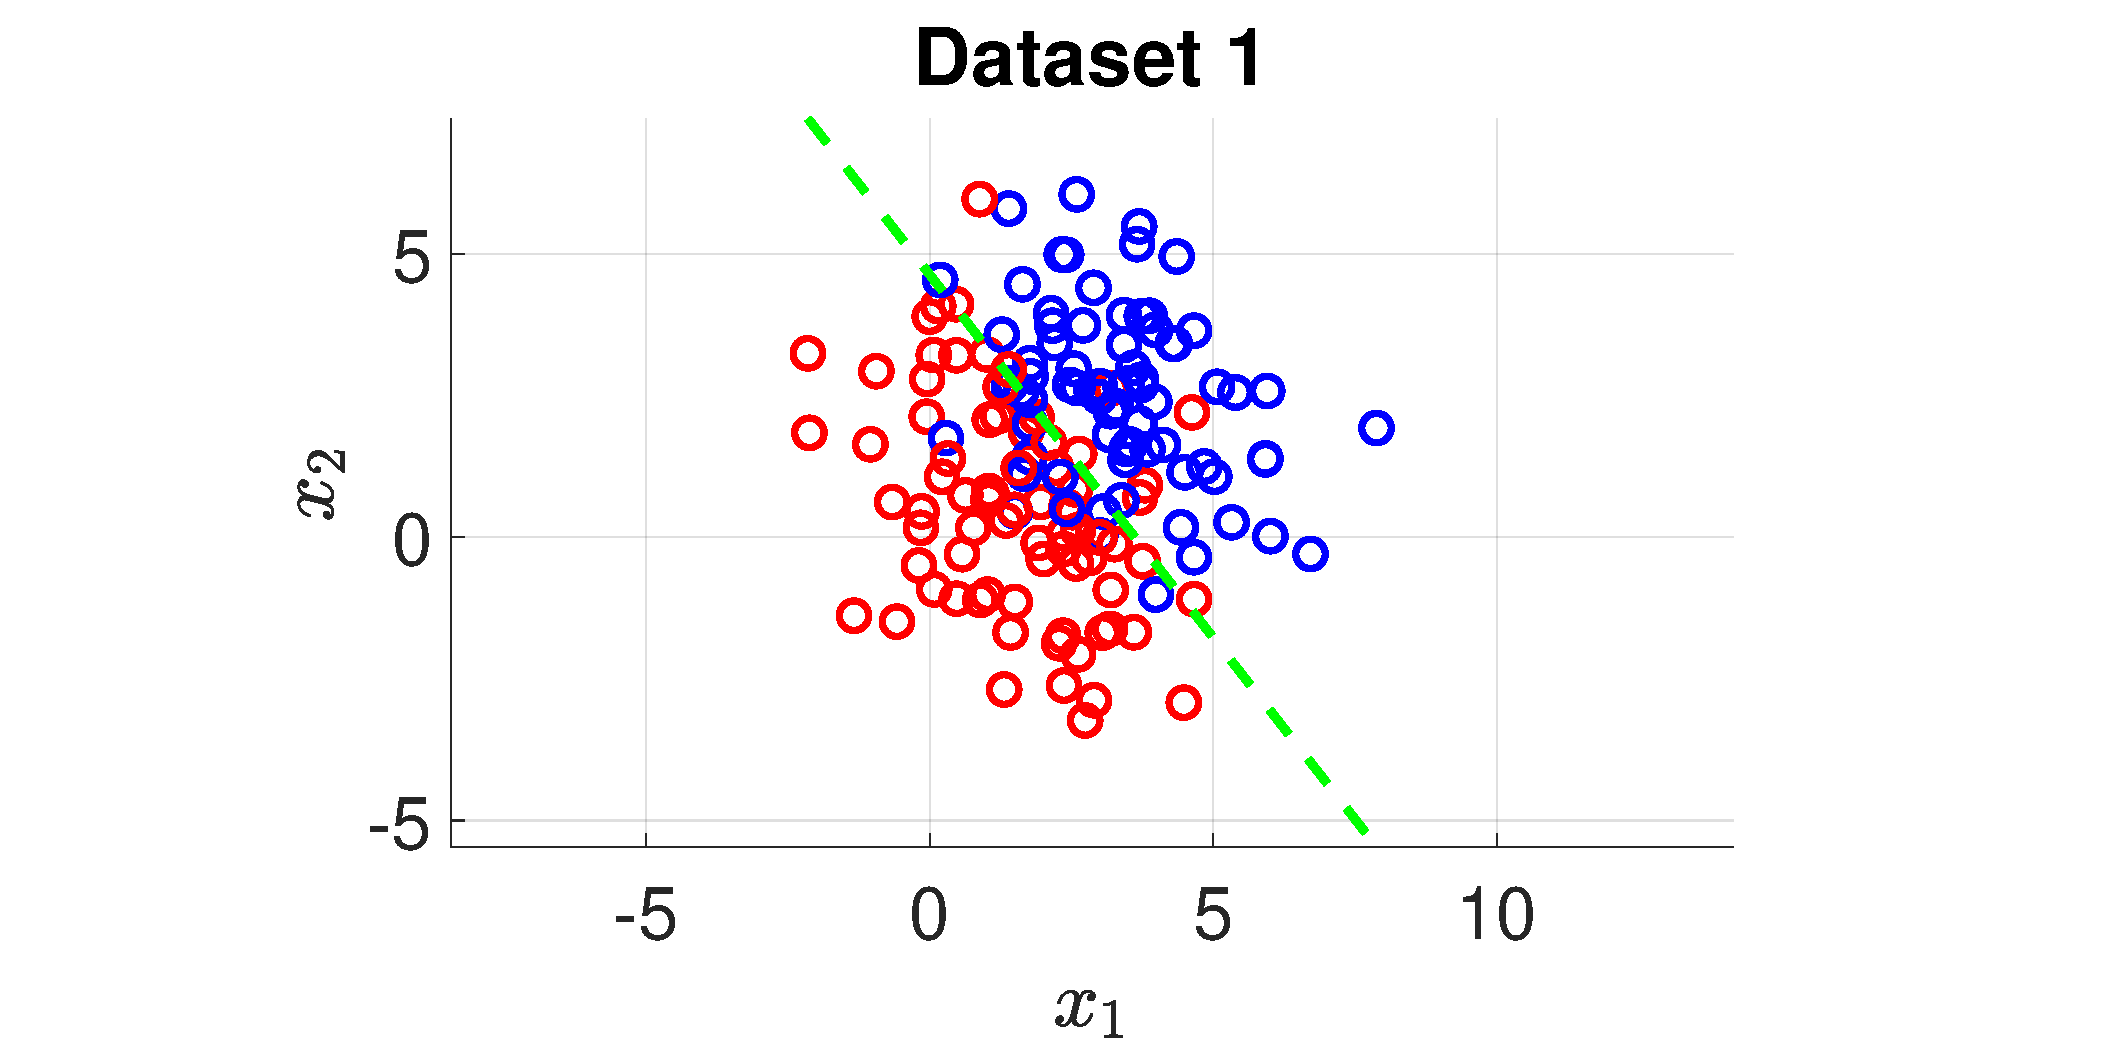
\includegraphics[width=\textwidth]{figures/GDsolDataset1.pdf}
    \caption{Dataset 1 and the corresponding line defined by $\{ x \in \mathbf{R}^2: s^T x = r\}$.}
    \label{fig:GD_dataset1}
\end{figure}

\begin{figure}[ht!]
    \centering
    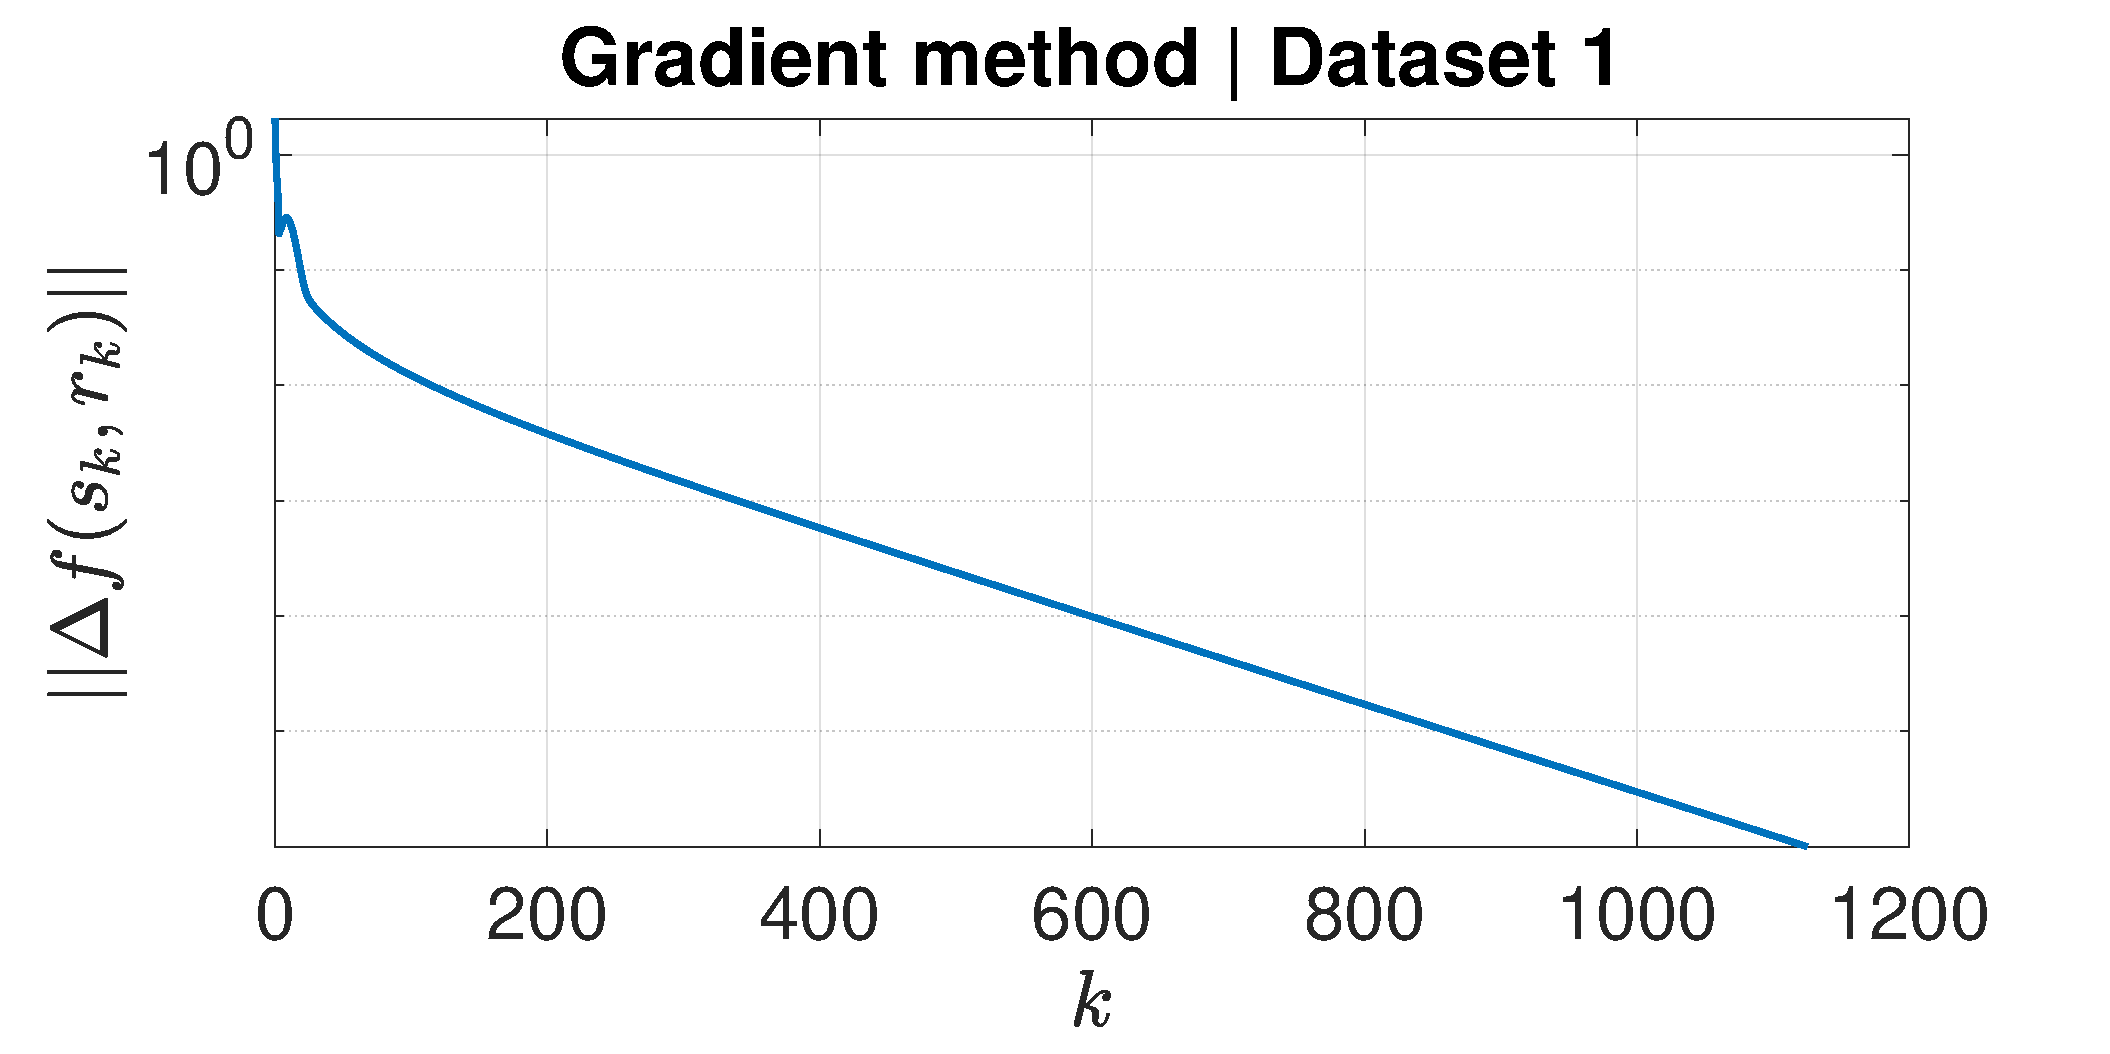
\includegraphics[width=\textwidth]{figures/GDNormGradDataset1.pdf}
    \caption{Norm of the gradient along iterations for the dataset 1.}
    \label{fig:GD_norm_dataset1}
\end{figure}

\subsection{Task 3}

In this Task, the code used was the one presented in the previous section. The results can be observed in Fig. \ref{fig:GD_dataset2} and \ref{fig:GD_norm_dataset2} and the values obtained for $s$ and $r$ were $s = (0.7402,2.3577)$ and $r=4.5553$.

\begin{figure}[ht!]
    \centering
    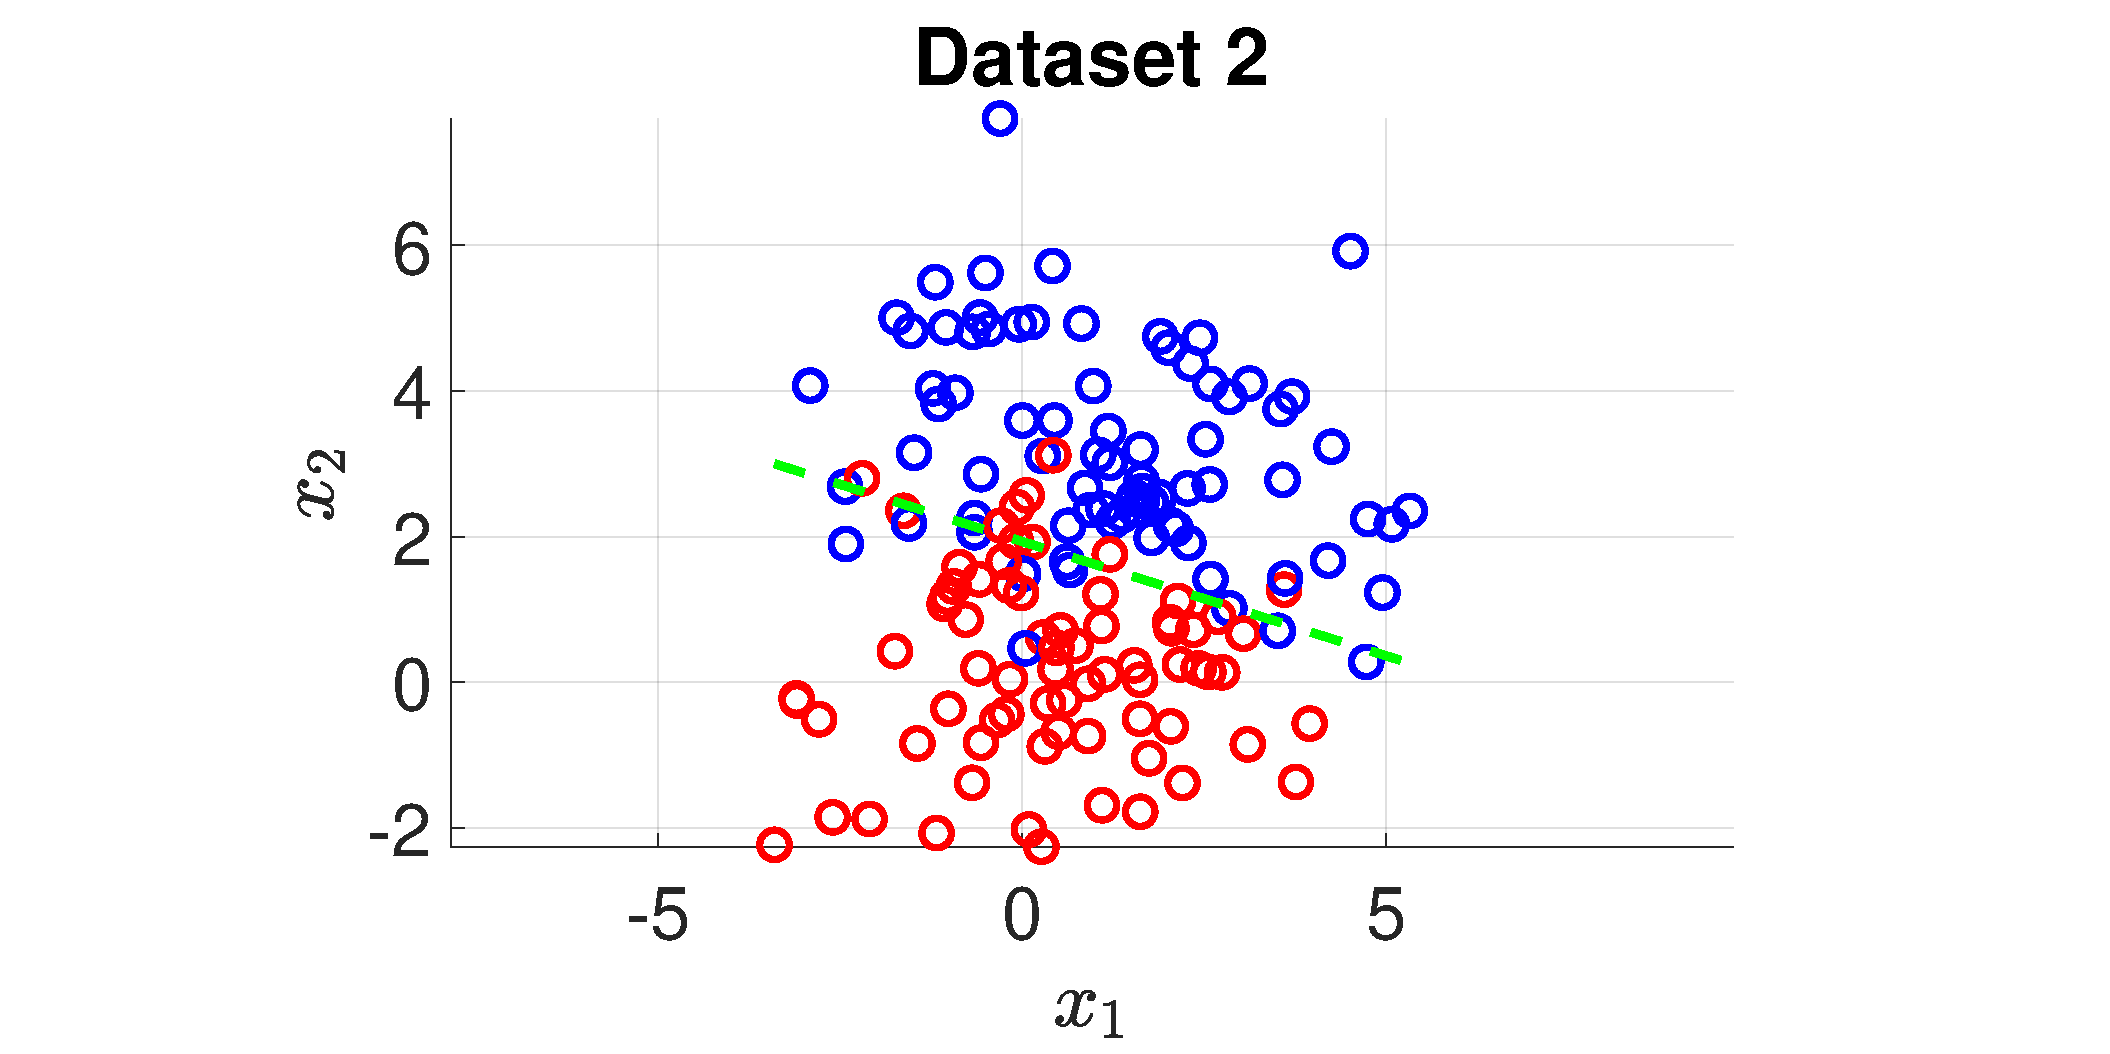
\includegraphics[width=\textwidth]{figures/GDsolDataset2.pdf}
    \caption{Dataset 2 and the corresponding line defined by $\{ x \in \mathbf{R}^2: s^T x = r\}$.}
    \label{fig:GD_dataset2}
\end{figure}

\begin{figure}[ht!]
    \centering
    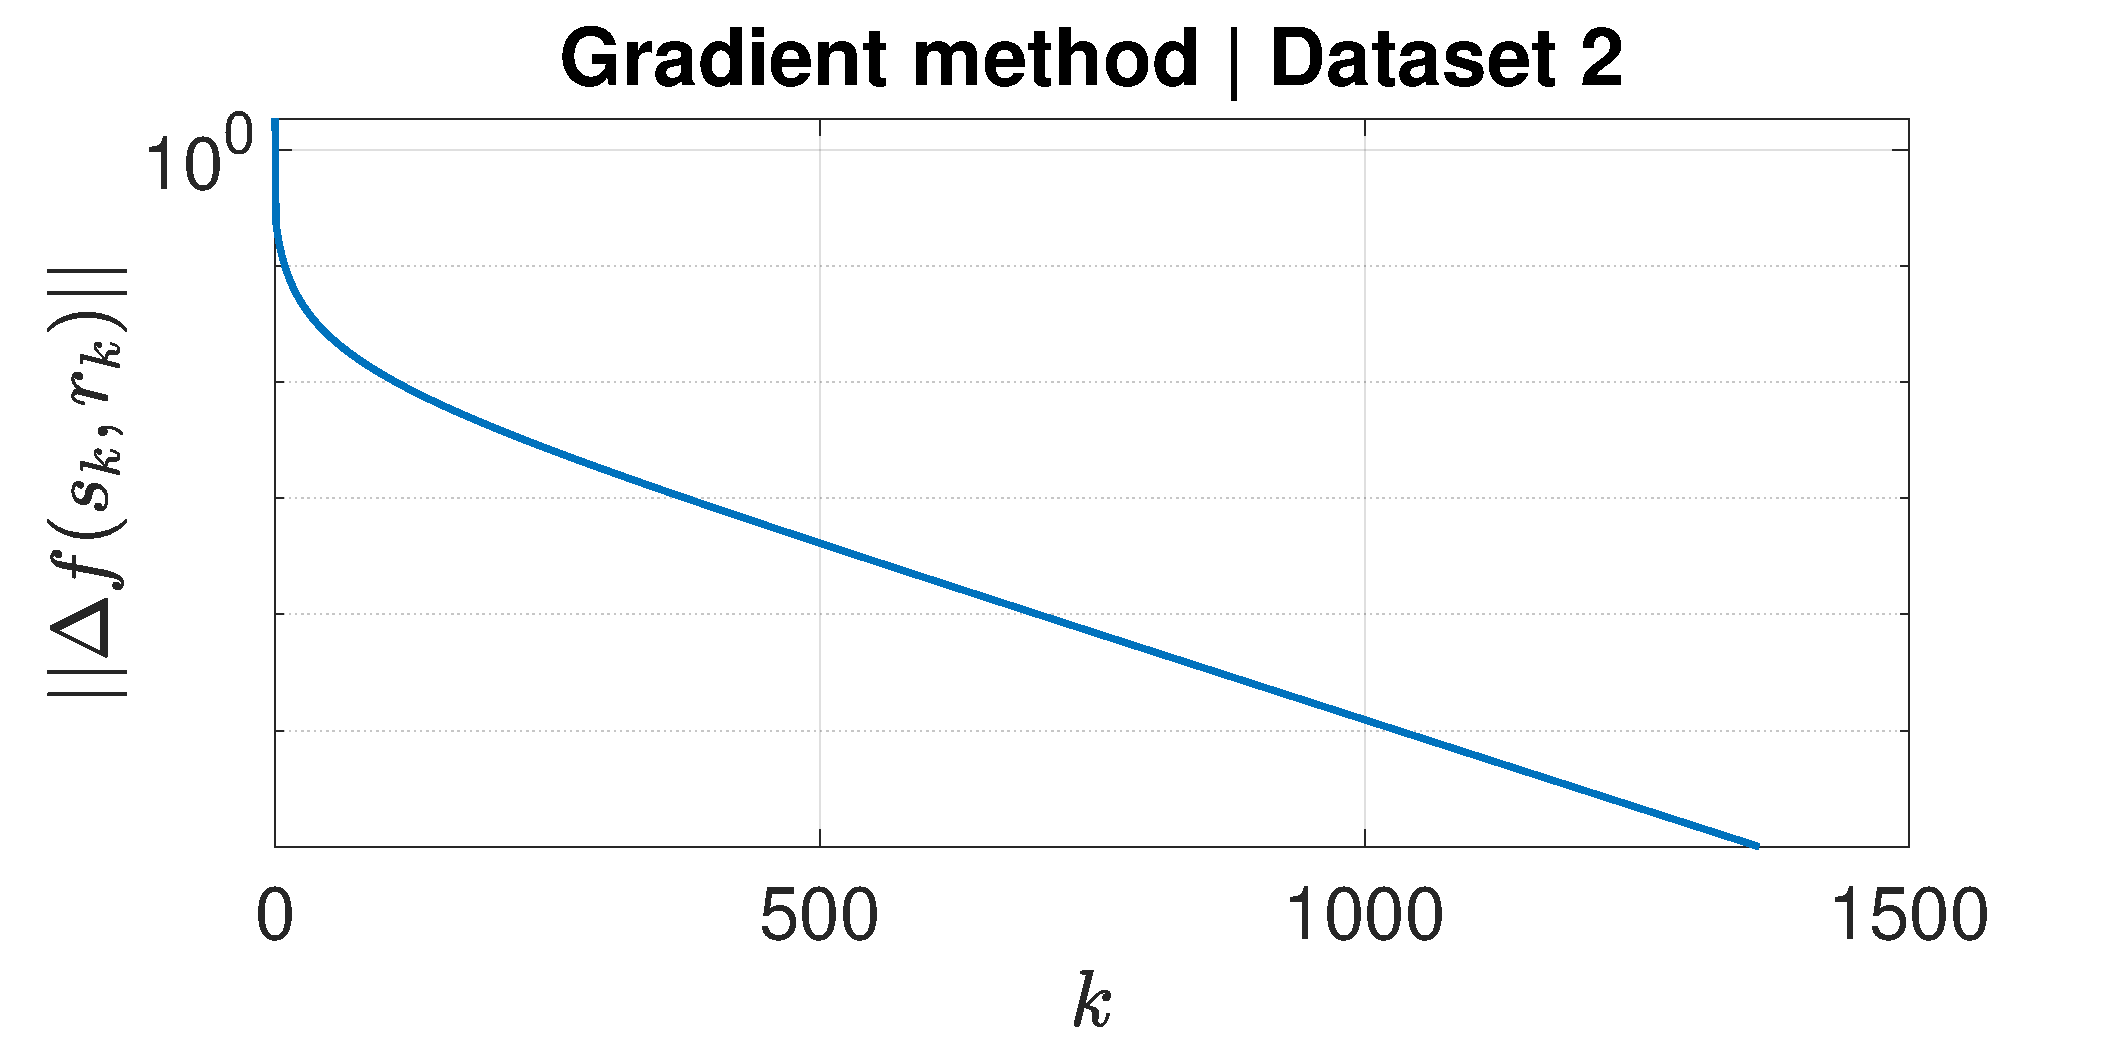
\includegraphics[width=\textwidth]{figures/GDNormGradDataset2.pdf}
    \caption{Norm of the gradient along iterations for the dataset 2.}
    \label{fig:GD_norm_dataset2}
\end{figure}

\subsection{Task 4}

In this Task, the gradient method was applied to two different datasets. However, in these datasets the points are no longer two-dimensional. In the dataset 3, $x_k \in \mathbf{R}^{30}$, for $k=1,...,500$, and in the dataset 4, $x_k \in \mathbf{R}^{100}$, for $k=1,...,8000$, which means it is no longer possible to represent the datasets. Therefore, only the global minimizers, $s$ and $r$, and the evolution of the norm of the gradient along iterations will be presented.

For dataset 3,
\begin{align*}
    s = [&-1.3082,1.4078,0.8049,-1.0024,0.5548,-0.5489,-1.1997,0.0792,-1.8279,-0.1484,\\
    &1.9241,-0.3586,-0.2900,0.1925,1.0614,0.2107,-0.0929,1.0476,-1.1248,-1.3311,\\
    &0.7661,-0.2729,-0.5349,0.9996,-0.4191,-0.3133,0.4075,-0.1965,-0.7379,\\
    &-0.9814],
\end{align*}
$r = 4.7984$, and the evolution of the norm of the gradient along iterations is represented in Fig. \ref{fig:GD_norm_dataset3}. For dataset 4,
\begin{align*}
    s = [&0.1098,
   -0.6423,
    0.1019,
    1.2428,
   -1.6431,
    1.0244,
    0.0512,
    0.8271,
    0.3136,
    0.7449,
   -0.5858,\\
    &0.6267,
    1.3611,
    0.1534,
    2.3234,
   -0.0840,
   -0.9489,
    2.4699,
   -0.8678,
   -1.6516,
    0.6460,\\
   &-0.4779,
    1.6397,
    0.9034,
   -1.2293,
   -0.7587,
   -0.4887,
    1.0306,
    0.0888,
   -1.0917,
   -1.2717,\\
   &-2.0333,
   -0.2505,
   -0.3518,
   -0.3486,
   -2.5610,
   -0.3132,
   -0.4902,
    0.7258,
    0.5774,\\
   &-1.0528,
    0.6400,
    0.3759,
   -0.1547,
    0.0298,
    0.9547,
   -0.2863,
    0.6364,
    0.7859,
    0.7584,\\
    &0.2880,
    0.1648,
    0.6776,
    2.0550,
    1.0996,
    0.5261,
   -0.5770,
    1.1454,
   -0.5617,
    0.0065,
    0.4768,\\
   &-2.3677,
   -1.1561,
   -2.6619,
    0.0622,
    0.1037,
   -0.6237,
    0.1913,
    0.6672,
   -1.0493,
   -0.3240,\\
   &-0.3207,
   -1.0904,
   -0.8293,
   -0.3104,
   -0.4879,
   -0.1060,
   -0.1646,
    2.2683,
   -1.2380,\\
   &-0.8575,
   -2.4781,
   -0.4158,
    0.1660,
    0.7931,
    0.3685,
   -0.0524,
   -0.9997,
   -0.5732,
    0.3971,\\
    &1.1911,
    1.8318,
   -1.7287,
    0.2329,
   -1.1921,
    1.6558,
    0.4612,
   -0.6431,
    0.8295,
    0.2975],
\end{align*}
$r = 7.6701$, and the evolution of the norm of the gradient along iterations is represented in Fig. \ref{fig:GD_norm_dataset4}.

\begin{figure}[ht!]
    \centering
    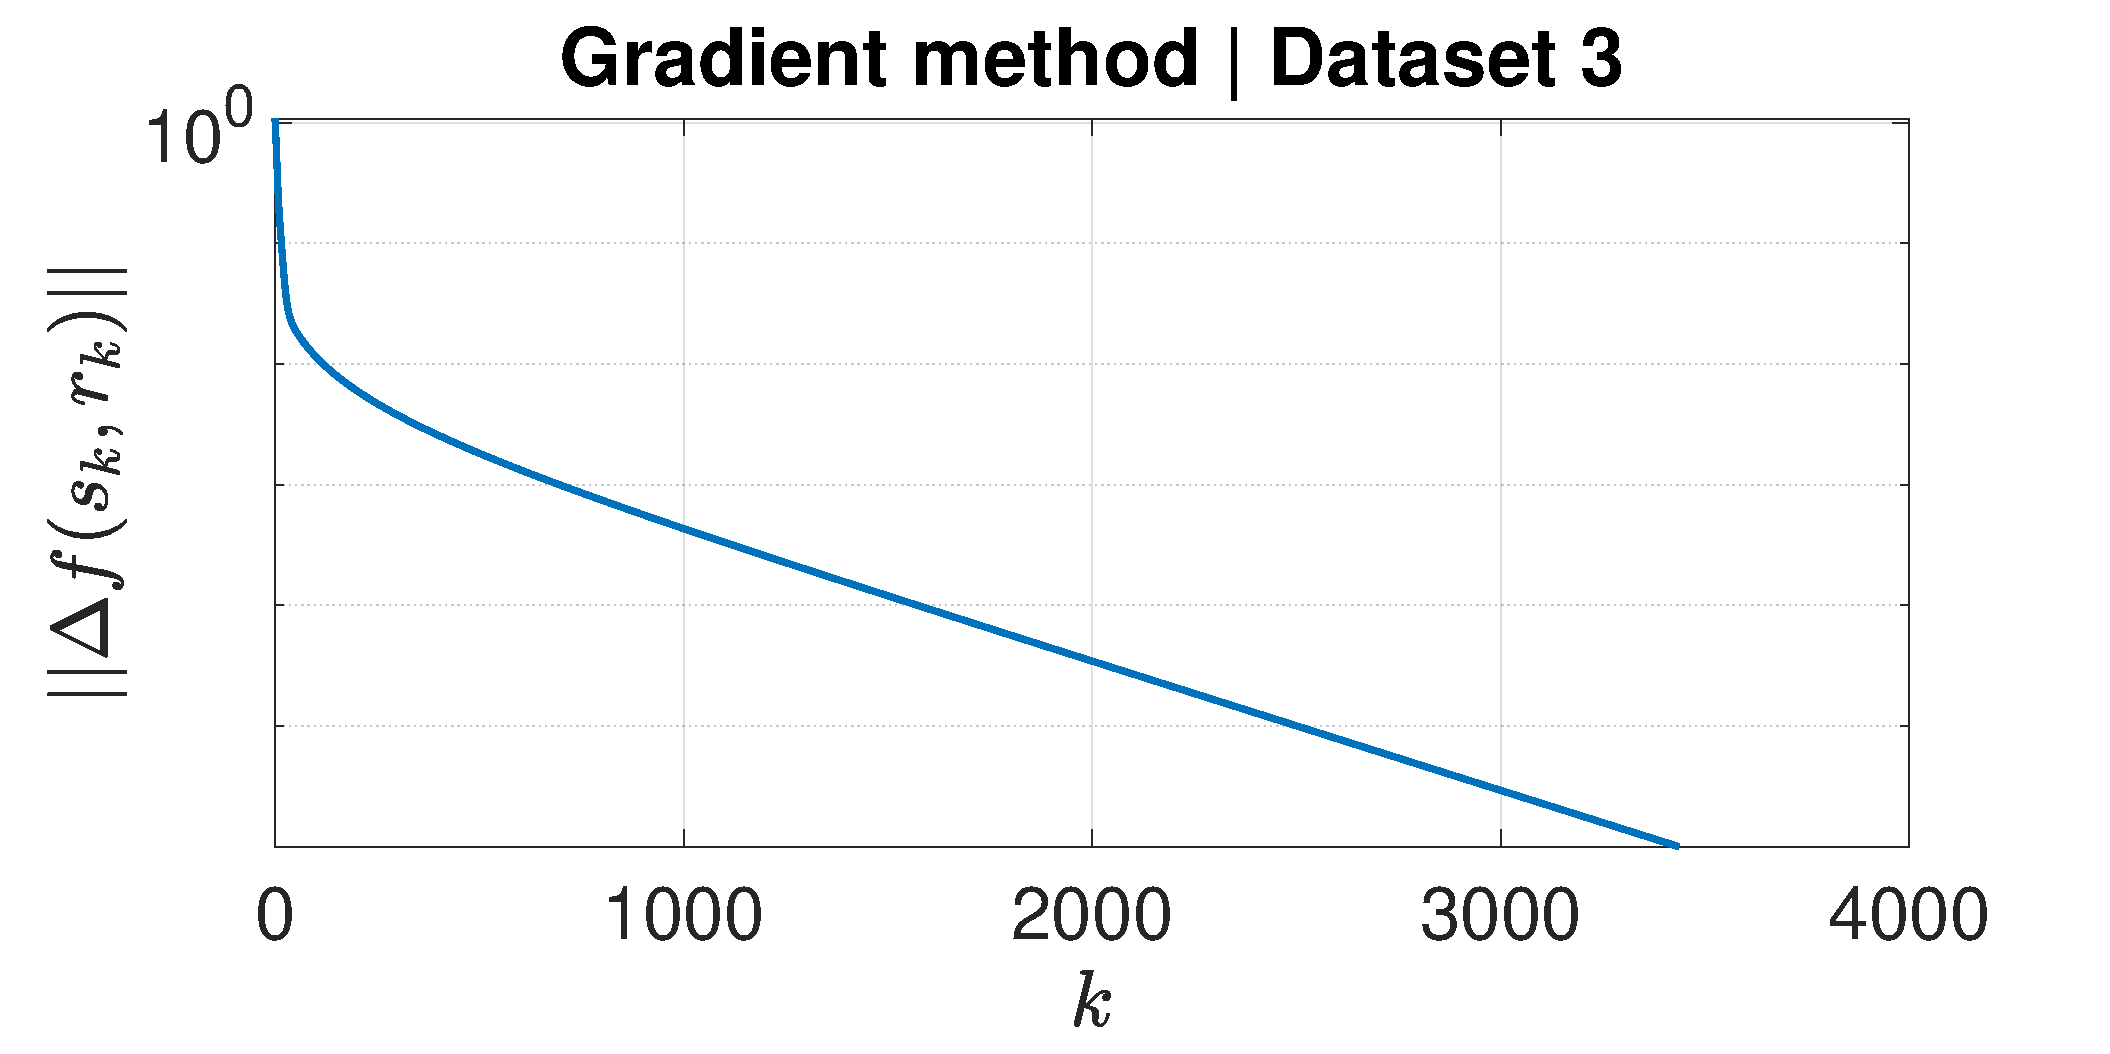
\includegraphics[width=0.9\textwidth]{figures/GDNormGradDataset3.pdf}
    \caption{Norm of the gradient along iterations for the dataset 3.}
    \label{fig:GD_norm_dataset3}
\end{figure}

\begin{figure}[ht!]
    \centering
    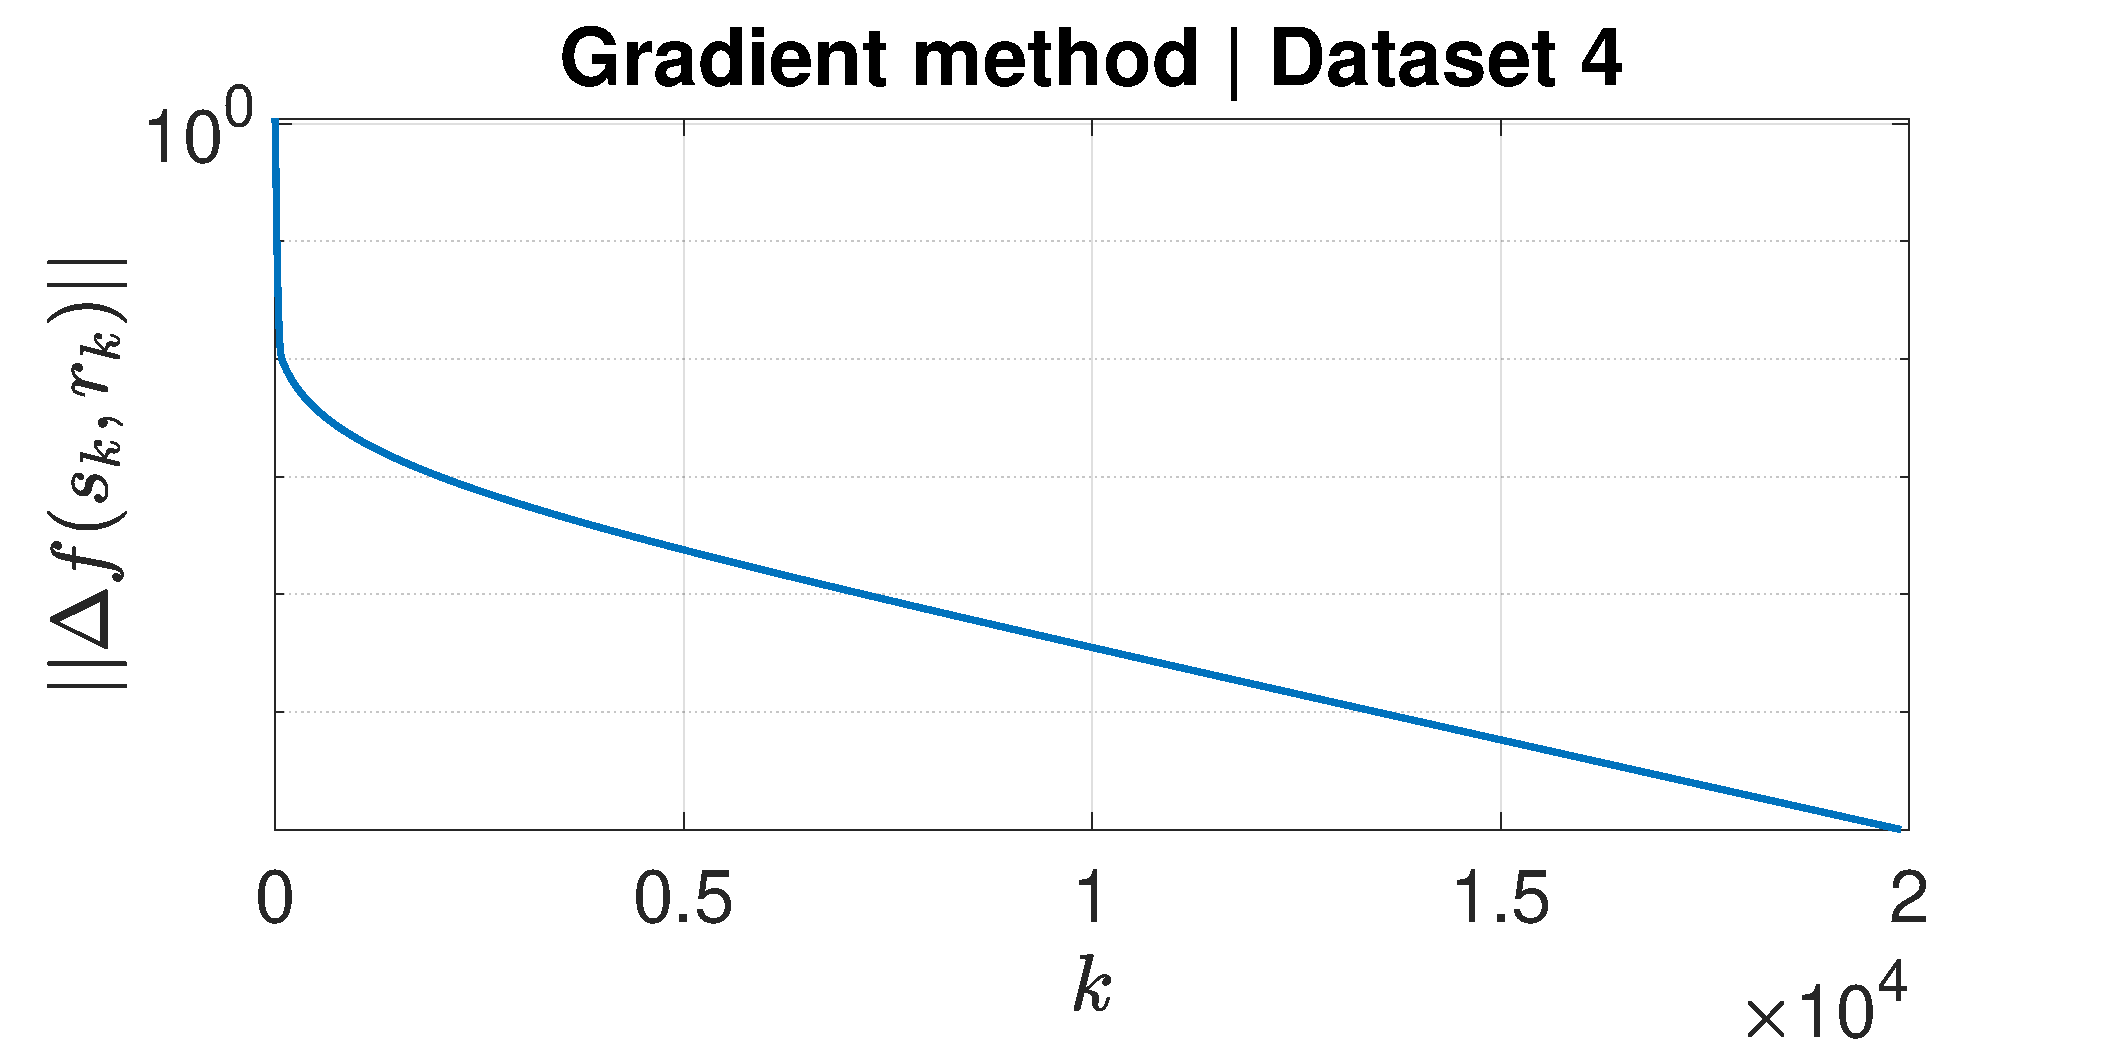
\includegraphics[width=0.9\textwidth]{figures/GDNormGradDataset4.pdf}
    \caption{Norm of the gradient along iterations for the dataset 4.}
    \label{fig:GD_norm_dataset4}
\end{figure}

\subsection{Task 5}

Letting $\phi: \mathbf{R} \rightarrow \mathbf{R}$ be a twice differentiable function and supposing $p: \mathbf{R}^3 \rightarrow \mathbf{R}$ is given by
\begin{equation} \label{eq:p}
    p(x) = \sum^K_{k=1} \phi \left(a_k^T x\right),
\end{equation}
where $a_k \in \mathbf{R}^3$ for $k = 1, ..., K$, one can write
\begin{equation} \label{eq:p_gradient}
    \nabla p (x) = \sum_{k=1}^K \dot{\phi}(a_k^T x) a_k = A v,
\end{equation}
where $A = [a_1 \quad a_2 \quad ... \quad a_K]$ and $v = [\phi(a_1^T x) \quad \phi(a_2^T x) \quad ... \quad \phi(a_K^T x)]^T$. In order to write the Hessian of $p$ at $x$, one can define, for $k=1,...,K$, the functions $u_k: \mathbf{R} \rightarrow \mathbf{R}^3$
\begin{equation} \label{eq:u}
    u_k(z) = z a_k,
\end{equation}
which, from \eqref{eq:p_gradient}, lead to
\begin{equation} \label{eq:p_gradient_u}
    \nabla p (x) = \sum_{k=1}^K u_k \left [\dot{\phi}(a_k^T x)\right].
\end{equation}
From \eqref{eq:u} and \eqref{eq:p_gradient_u}, it is possible to write
\begin{equation} \label{eq:p_hessian}
    \nabla^2 p(x) = \sum_{k=1}^K D u_k \left [\dot{\phi}(a_k^T x)\right] D \left [\dot{\phi}(a_k^T x) \right] D(a_k^T x) = \sum_{k=1}^K a_k \ddot{\phi}(a_k^T x) a_k^T = A D A,
\end{equation}
where D is the diagonal matrix
\begin{equation} \label{eq:p_hessian_D}
    D = 
    \begin{bmatrix}
    \ddot{\phi}(a_1^T x) &&& \\
    & \ddot{\phi}(a_2^T x) && \\
    &&...&\\
    &&& \ddot{\phi}(a_K^T x) \\
    \end{bmatrix}
\end{equation}

\subsection{Task 6}

In this Task, the Newton method will be used to solve \eqref{eq:problem}. To be able to use this method, it is necessary to know the gradient, which is given by \eqref{eq:gradient_final}, and the Hessian of the objective function. In order to write the Hessian, one starts by writing, from \eqref{eq:objective_function_task_1}, \eqref{eq:hk_0}, and \eqref{eq:lk},
\begin{equation} \label{eq:new_f}
    f(x) = \sum_{k=1}^K \left (\phi \left (a_k^T x \right) + \frac{1}{K} \begin{bmatrix}
    -y_k x_k \\
    y_k
    \end{bmatrix}^T x \right),
\end{equation}
where $x = [s \quad r]^T$, $a_k = [x_k \quad -1]^T$ and $\phi:\mathbf{R} \rightarrow \mathbf{R}$
\begin{equation} \label{eq:new_phi}
    \phi (z) = \frac{1}{K}\log (1 + \exp (z))
\end{equation}
with second-derivative
\begin{equation} \label{eq:phi_second_d}
    \ddot{\phi} (z) = \frac{\exp(z)}{K \left[1+\exp(z)\right]^2}.
\end{equation}
Taking into consideration that \eqref{eq:new_f} is written in the form of \eqref{eq:p} except for the sum of affine therms whose second-derivative is null, it may be written, from \eqref{eq:p_hessian}, \eqref{eq:p_hessian_D}, and \eqref{eq:phi_second_d},
\begin{equation} \label{eq:hessian_final}
    \nabla^2 f(x) = \begin{bmatrix}
    a_1 & a_2 & ... & a_K
    \end{bmatrix} 
    \begin{bmatrix}
    \ddot{\phi}(a_1^T x) &&& \\
    & \ddot{\phi}(a_2^T x) && \\
    &&...&\\
    &&& \ddot{\phi}(a_K^T x) \\
    \end{bmatrix}
    \begin{bmatrix}
    a_1 & a_2 & ... & a_K
    \end{bmatrix}.
\end{equation}

Taking into consideration \eqref{eq:gradient_final} and \eqref{eq:hessian_final}, the Newton method was implemented according to the script below. In it, the Newton algorithm is implemented through the MATLAB function \textit{newtonAlgorithm} also presented below.

\subsection{Task 7}

\section{Part 3}

\end{document}